\chapter{Sets and Maps}

A \textbf{Set} is one of the most basic structures we can construct in mathematics.

\begin{definition}[Set]
  A set is a collection of indistinguiable objects.
\end{definition}

The simplest set is the null set $ \emptyset = \{ \}$, the set that contains no objects.

Or we could have a set with one object, like $\{ \emptyset \}$, or $\{$\ding{36} $\}$.

We have two basic operations we can perform on sets, union and intersection.

\begin{definition}[Union]
  $c \in A \cup B$ if $a \in  A$ \textbf{OR} $a \in B$. $A\cup B$ is called the \textbf{union} of $A$ and $B$.
\end{definition}

\begin{definition}[Intersection]
  $c \in A \cap B$ if $a \in B$ \textbf{AND} $a \in B$.  $A \cap B$ is called the \textbf{intersection} of $A$ and $B$.
\end{definition}

Time for some examples:

Let $A = \{$\ding{40},\ding{88},\ding{101},\ding{161}$\}$ and $B= \{$ \ding{40}, \ding{39} $\}$.

Then $A \cup B = \{$\ding{40},\ding{88},\ding{101},\ding{161},\ding{39} $\}$.  And $A\cap B = \{$ \ding{40} $\}$.

You might notice I'm using weird shapes instead of numbers as members of my sets.  I don't want you to get stuck into thinking that these definitions and concepts only apply to abstract numbers and the sorts of things you dealt with in high school.  An investigator might very well look for the \textit{intersection} of those who where at Jimmy's bar on Friday night and The Pit on Saturday.  LGBTQ stands for the \textit{union} of Lesbians, Gays, Bisexuals, Transgenders, and Queers.

Seems fairly straightforward. But everything after that we do will be built on having a solid foundation in sets.

\begin{table}
\begin{tabular}{| c | c | c |}
  \hline
  Notation & Name & Example Elements \\
  \hline
  $\mathbb{R}$ & the Real line & 1, $\pi$, $\sqrt{2}$, $569543/3874329$, and $.3234898957786...$ \\
   $\mathbb{Z}$ & the Integers &  $-1, 0, 1, 2,...$ \\
  $\mathbb{Q}$ & The Rationals & $p/q : p,q \in \mathbb{Z}$ \\
  $S^1$ &  The surface of a circle. & $e^{i \phi} $ \\
  $S^2$ & The surface of a sphere. & \\
  \hline
\end{tabular}
  \caption{The names of some common special sets often encountered.}
  \label{tab:sets}
\end{table}



  Modern mathematics attempts to build up as much as possible just from sets.  Even our ideas of numbers

When we restrict our discussion of equivalence to just maps between sets, we get two important definitions,

\begin{definition}[Homomorphism]
  Given two sets $X$ and $Y$ with an algebraic structure on them $\circ$ , for example mulitplication, and a map between them $\phi:X\rightarrow Y$, $\phi$ is called a \textbf{homomorphism} and $X$ and $Y$ are said to be \textbf{homomorphic} to each other if $\phi$ preserves the structure on $Y$.  In other words, for $x_1,x_2 \in X$, $\phi(x_1)\circ \phi(x_2) = \phi(x_1 \circ x_2) \in Y$.
\end{definition}

Homomorphism just goes one way.  If we have this property in both directions, $X\rightarrow Y$ and $Y\rightarrow X$ we use the stricter condition of \textbf{Isomorphism},

\begin{definition}[Isomorphism]
  Given two sets $X$ and $Y$ with an algebraic structure on them $\circ$ and a map between them $\phi:X\rightarrow Y$, $\phi$ is called a \textbf{isomorphism} and $X$ and $Y$ are said to be \textbf{isomorphic} to each other if $\phi$ is homomorphic, and there exists an inverse $\phi^{-1}: Y \rightarrow X$ that is also homomorphic.
\end{definition}

\begin{figure}
  \begin{subfigure}{.25\textwidth}
    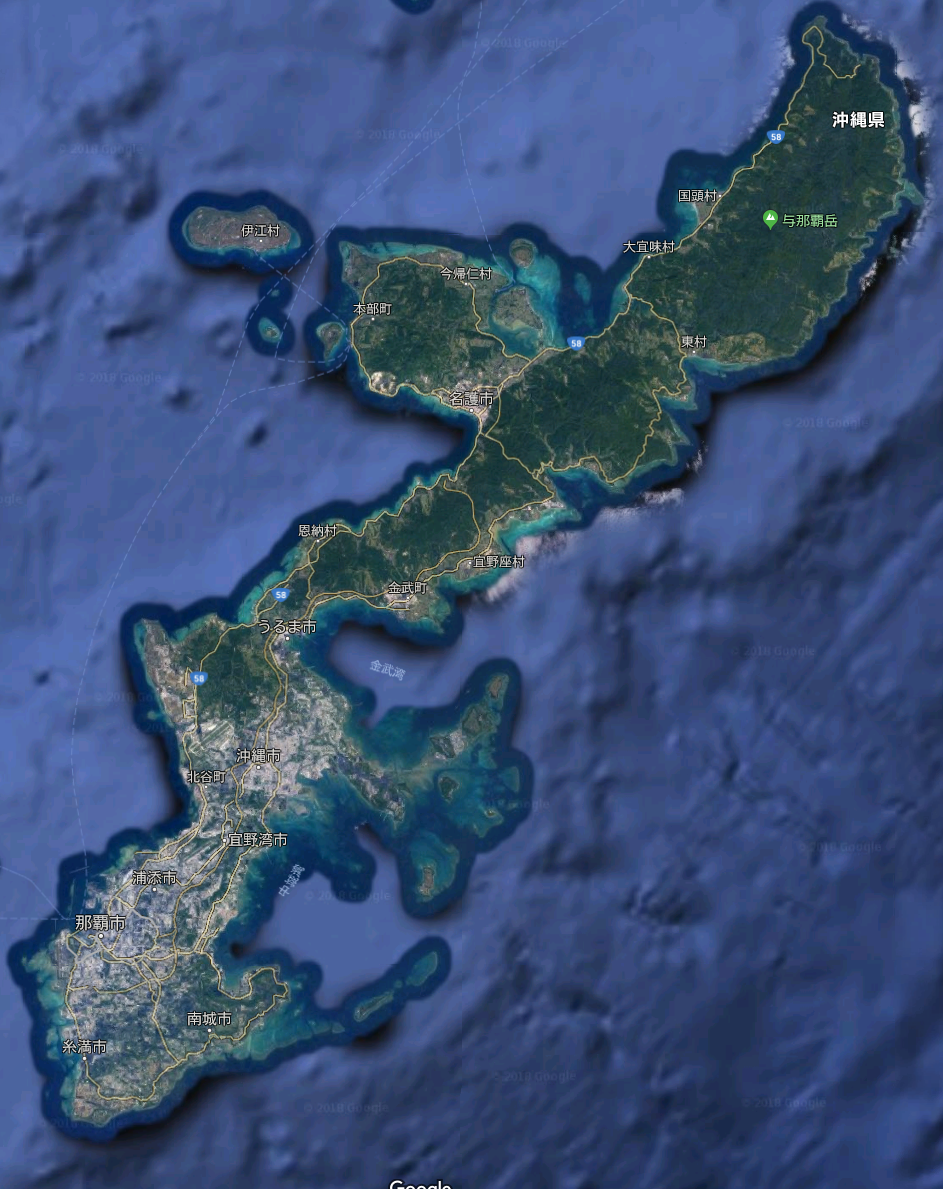
\includegraphics[width=\textwidth]{pics/okinawa.png}
    \caption{}
    \label{fig:okinawa}
  \end{subfigure}
  \begin{subfigure}{.25\textwidth}
    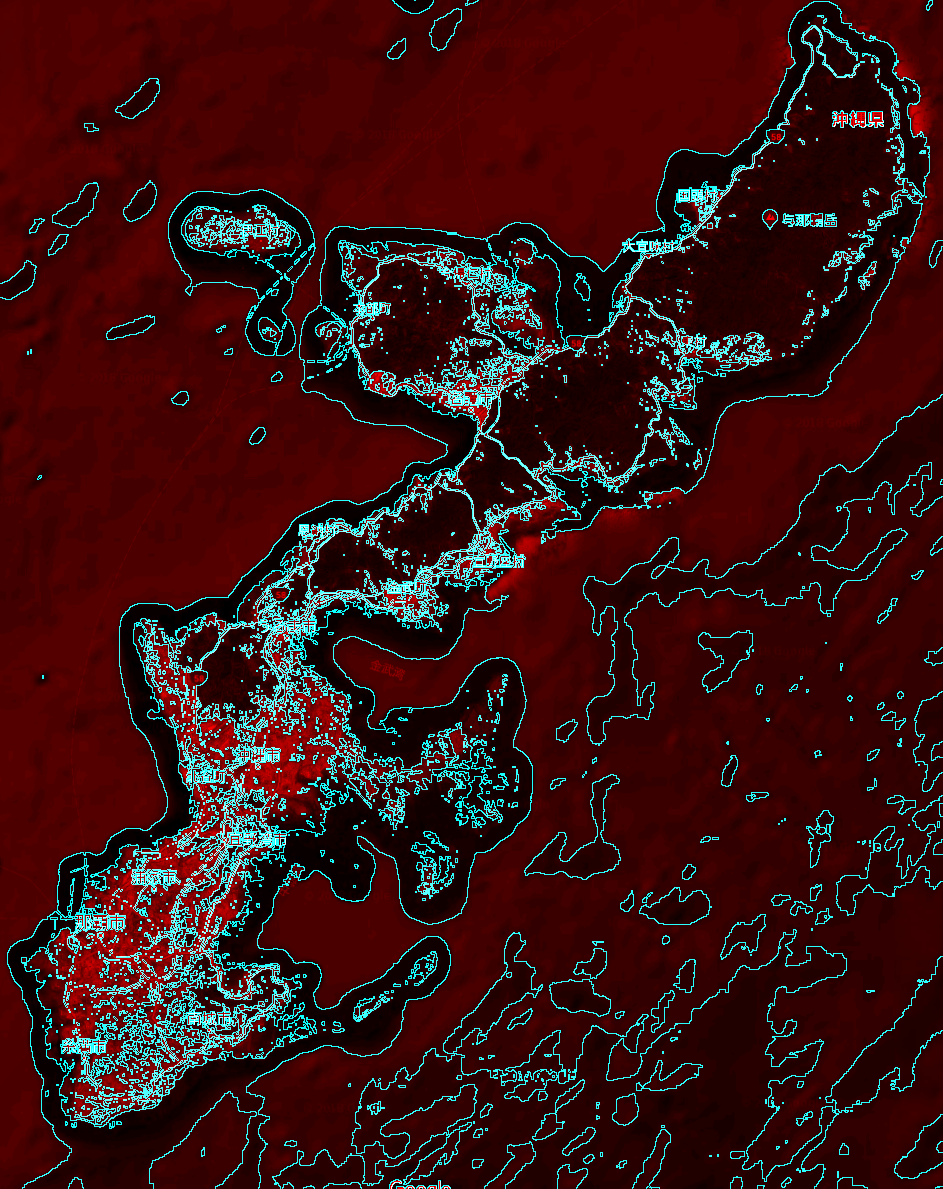
\includegraphics[width=\textwidth]{pics/okinawa_lines.png}
    \caption{}
    \label{fig:okinawa_lines}
  \end{subfigure}
  \begin{subfigure}{.25\textwidth}
    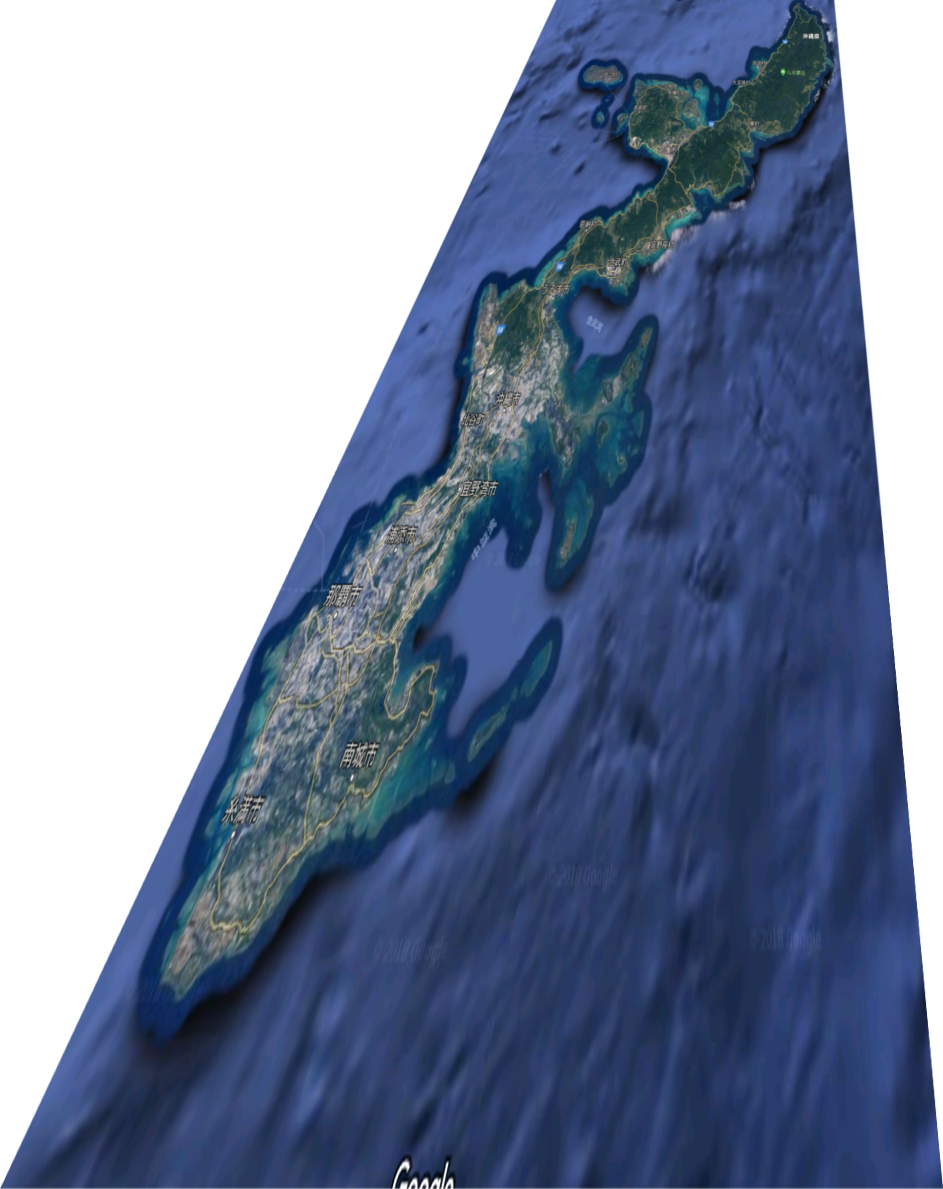
\includegraphics[width=\textwidth]{pics/okinawa_distort.png}
    \caption{}
    \label{fig:okinawa_distort}
  \end{subfigure}
  \caption{\ref{fig:okinawa} and \ref{fig:okinawa_lines} are only homomorphic to each other, since \ref{fig:okinawa} cannot be reconstructed from \ref{fig:okinawa_lines}.  \ref{fig:okinawa} and \ref{fig:okinawa_distort} are isomorphic in addition to being homomorphic since they are merely distortion of each other.  No information was lost.  }
\end{figure}
